\chapter{Optimization and Statistics} \label{chp:optimization}
\epigraph{Great quote.}{Author}
\begin{figure}[H]
	\centering
	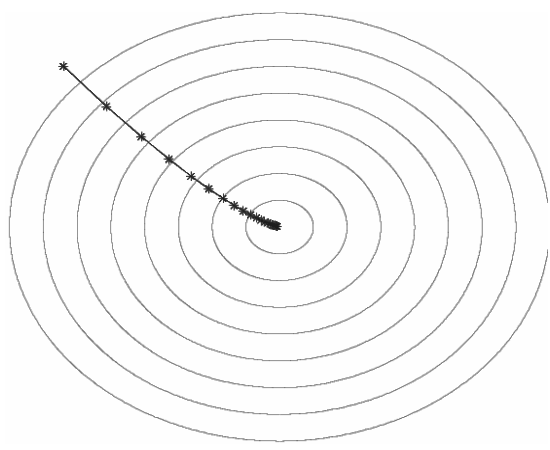
\includegraphics[scale=0.5]{Images/gd_bw.png}
	\caption{An iterative optimization algorithm is always approaching an extremum in a possibly multi-dimensional space. Here illustrated in a two-dimensional space where the equipotential curves are drawn.}
\end{figure}

Optimization is a wide term..

\newpage
\section{Optimization algorithms}
In chapter \ref{chp:machinelearning}, we discussed the gradient descent optimization algorithm, which is among the most basic methods available. That method is based on the gradient, which is the slope of the cost function, but many methods are also in need of the Hessian matrix, which gives the curvature of the cost function. We will barely scratch the surface of this field, limiting us to the gradient methods. 

To have the method fresh in mind, we will start with reintroducing the gradient descent method before we move on the its stochastic brother. We will then have a look at how momentum can be added, and finally we examine the stochastic and momentum based ADAM optimizer. 

\subsection{Gradient descent} \label{sec:gd}
Perhaps the simplest and most intuitive method for finding the minimum is the gradient descent method, which reads
\begin{empheq}[box={\mybluebox[5pt]}]{align}
\label{eq:GD}
\theta_t^i=\theta_{t-1}^i - \eta\frac{\partial \mathcal{C}(\bs{\theta}_{t-1})}{\partial\theta^i}
\end{empheq}
where $\theta_t^i$ is the parameter $\theta^i$ at time step (iteration) $t$ and $\eta$ is the learning rate. The idea is to find in which direction the cost function $\mathcal{C}(\bs{\theta})$ has the steepest slope, and move in the direction which minimizes the cost function. For every time step, the cost function is thus minimized, and when the gradient approaches zero the minimum is found. A possible stop criterion is
\begin{equation}
\frac{\partial \mathcal{C}(\bs{\theta})}{\partial\theta^i}<\varepsilon.
\end{equation}
where $\varepsilon$ is a tolerance. 

In cases where the cost function is not strictly decreasing, we will have both local and global minima. Often, it is hard to say whether we are stuck in a local or global minimum, and this is where the stochasticity enters the game.

\subsection{Stochastic gradient descent}
Stochastic gradient descent is closely related to the gradient descent method, but the method uses randomly selected batches to evaluate the gradients, hence the stochasticity. By introducing this randomness, the parameters will not always be updated in order to minimize the energy, which makes the us less likely to be stuck in a local minimum.

In practice, one splits the data set into $n$ batches, and select one of them to be used in the parameter update. Our hope is that this batch is representative for the entire data set, such that the new parameters gives a lower cost function. If that is the case, we have reduced the cost of an iteration, significantly, since we only need to care about a batch. After each batch in the data set has had an opportunity to update the internal parameters, we say that we have performed an \textit{epoch}.

We are not guaranteed that updating the parameters with respect to a batch gives a lower cost function, and when it is not, we need to run more batches in order to minimize the cost function. Since each epoch is faster than for standard gradient descent, this is acceptable. As long as the batch is slightly representative for the entire data set, the cost function will be minimized in the end.

Mathematically, we the method can be expressed as 
\begin{empheq}[box={\mybluebox[5pt]}]{align}
\label{eq:SGD}
\theta_t^i=\theta_{t-1}^i - \eta\frac{\partial \mathcal{C}_k(\bs{\theta}_{t-1})}{\partial\theta^i}
\end{empheq}
where we use the $k$'th batch in the parameter update. Standard gradient descent is actually just a special case of this, where we only have one batch ($k$ includes the whole data set). If we still get stuck in local minima after adding the stochasticity, it might be a good idea to add momentum as well.

\subsection{Adding momentum} \label{sec:momentum}
If we go back to an introductory mechanics course, you might remember that momentum is a quantity that maintains the motion of a body. Imagine a ball that rolls down a steep hill, but then there is a local minimum that it needs to escape to keep rolling. If it has enough momentum, it will be able to escape.

Exactly the same idea lies behind the momentum used in optimization algorithms; the momentum will try to maintain the motion towards the global minimum, which makes the system less likely to be stuck in a local minimum.  

Momentum can be added to most optimization algorithms, also gradient descent and stochastic gradient descent. The way we do it is to save the direction we were moving in the previous iteration, and use it as a contribution to the next gradient update. A typical implementation of the first-order momentum looks like
\begin{empheq}[box={\mybluebox[5pt]}]{align}
m_t^i &= \gamma m_{t-1}^i + \eta\frac{\partial \mathcal{C}(\bs{\theta}_{t-1})}{\partial\theta^i}\\
\theta_t^i&=\theta_{t-1}^i-m_t^i
\end{empheq}
where $\gamma$ is the momentum parameter, which is just another hyper parameter. $\gamma$ is usually set to a small number, and initially we set all $m_0^i=1$.

The optimization algorithm can be modified further in unlimited ways. A common improvement is to add higher order momentum, another is to make the learning rate adaptive. We have implemented the most basic version of this, with monotonic adaptivity. Many algorithms also make use of the Hessian, as discussed in the introduction, but that is another level. We will end this section with setting up the algorithm of a stochastic gradient descent optimization with momentum and monotonic adaptivity. 
\begin{algorithm}[H]
	\SetAlgoLined
	\KwData{this text}
	\KwResult{how to write algorithm with \LaTeX2e }
	initialization\;
	\While{not at end of this document}{
		read current\;
		\eIf{understand}{
			go to next section\;
			current section becomes this one\;
		}{
			go back to the beginning of current section\;
		}
	}
	\caption{Adaptive stochastic gradient descent with momentum}
\end{algorithm}

\subsection{ADAM}
ADAM is a first-order stochastic optimization method which is widely used in machine learning. It was discovered by D.P. Kingma and J. Ba, and published in a 2014 paper. The article has already more than 25000 citations! \cite{kingma_adam:_2014} So what makes this method so popular? 

The main reason why it is widely used, is obviously that it performs good. The fact that it only requires the gradient makes it efficient, and the way the momentum is implemented still makes able to handle a large number of parameters. 

The optimization algorithm can be expressed as a set of difference equations
\begin{empheq}[box={\mybluebox[5pt]}]{align}
g_t^i&=\frac{\partial \mathcal{C}(\bs{\theta}_{t-1})}{\partial\theta^i}\notag\\
m_t^i&=\gamma_1m_{t-1}^i+(1-\gamma_1)g_t^i\notag\\
v_t^i&=\gamma_2v_{t-1}^i+(1-\gamma_2)(g_t^i)^2\notag\\
\hat{m}_t^i&=m_t^i/(1-\gamma_1^t)\\
\hat{v}_t^i&=v_t^i/(1-\gamma_2^t)\notag\\
\theta_t^i&=\theta_{t-1}^i-\eta\hat{m}_t^i/(\sqrt{\hat{v}_t^i}+\varepsilon)\notag
\end{empheq}
where $m_t^i$ is the biased first momentum estimate if parameter $\theta_i$ and $v_t^i$ is the biased second raw moment estimate. The momentum parameters $\gamma_1$ and $\gamma_2$ need to be in the range $\gamma_j\in[0,1)$, and are often set to values close to 1. This makes the optimization adaptive: as time goes, the factors $1-\gamma_j^t$ approach 1 from below. $\eta$ corresponds to the learning rate, and should be a small number. Finally, the parameter $\varepsilon$ is added to avoid division by zero. 

The algorithm goes as following

\begin{algorithm}[H]
\SetAlgoLined
\KwData{this text}
\KwResult{how to write algorithm with \LaTeX2e }
initialization\;
\While{not at end of this document}{
	read current\;
	\eIf{understand}{
		go to next section\;
		current section becomes this one\;
	}{
		go back to the beginning of current section\;
	}
}
\caption{The ADAM algorithm}
\end{algorithm}

\section{Variance estimation}
\begin{equation}
\sigma^2=\langle E_L^2\rangle - \langle E_L\rangle^2
\end{equation}

\section{Resampling analysis} \label{sec:resampling}
\subsection{Blocking}
dkdkdk



\section{Random number generators} \label{sec:RNG}
In the Monte-Carlo sampling we are drawing millions of numbers, and in order to get accurate estimations, they should all be random, independent and fast to get. 

In C++ there are plenty of random number generator available, but not all of them meet our requirements. For instance the standard 

Mersenne Twister needs to be mentioned here